\documentclass[1p]{elsarticle_modified}
%\bibliographystyle{elsarticle-num}

%\usepackage[colorlinks]{hyperref}
%\usepackage{abbrmath_seonhwa} %\Abb, \Ascr, \Acal ,\Abf, \Afrak
\usepackage{amsfonts}
\usepackage{amssymb}
\usepackage{amsmath}
\usepackage{amsthm}
\usepackage{scalefnt}
\usepackage{amsbsy}
\usepackage{kotex}
\usepackage{caption}
\usepackage{subfig}
\usepackage{color}
\usepackage{graphicx}
\usepackage{xcolor} %% white, black, red, green, blue, cyan, magenta, yellow
\usepackage{float}
\usepackage{setspace}
\usepackage{hyperref}

\usepackage{tikz}
\usetikzlibrary{arrows}

\usepackage{multirow}
\usepackage{array} % fixed length table
\usepackage{hhline}

%%%%%%%%%%%%%%%%%%%%%
\makeatletter
\renewcommand*\env@matrix[1][\arraystretch]{%
	\edef\arraystretch{#1}%
	\hskip -\arraycolsep
	\let\@ifnextchar\new@ifnextchar
	\array{*\c@MaxMatrixCols c}}
\makeatother %https://tex.stackexchange.com/questions/14071/how-can-i-increase-the-line-spacing-in-a-matrix
%%%%%%%%%%%%%%%

\usepackage[normalem]{ulem}

\newcommand{\msout}[1]{\ifmmode\text{\sout{\ensuremath{#1}}}\else\sout{#1}\fi}
%SOURCE: \msout is \stkout macro in https://tex.stackexchange.com/questions/20609/strikeout-in-math-mode

\newcommand{\cancel}[1]{
	\ifmmode
	{\color{red}\msout{#1}}
	\else
	{\color{red}\sout{#1}}
	\fi
}

\newcommand{\add}[1]{
	{\color{blue}\uwave{#1}}
}

\newcommand{\replace}[2]{
	\ifmmode
	{\color{red}\msout{#1}}{\color{blue}\uwave{#2}}
	\else
	{\color{red}\sout{#1}}{\color{blue}\uwave{#2}}
	\fi
}

\newcommand{\Sol}{\mathcal{S}} %segment
\newcommand{\D}{D} %diagram
\newcommand{\A}{\mathcal{A}} %arc


%%%%%%%%%%%%%%%%%%%%%%%%%%%%%5 test

\def\sl{\operatorname{\textup{SL}}(2,\Cbb)}
\def\psl{\operatorname{\textup{PSL}}(2,\Cbb)}
\def\quan{\mkern 1mu \triangleright \mkern 1mu}

\theoremstyle{definition}
\newtheorem{thm}{Theorem}[section]
\newtheorem{prop}[thm]{Proposition}
\newtheorem{lem}[thm]{Lemma}
\newtheorem{ques}[thm]{Question}
\newtheorem{cor}[thm]{Corollary}
\newtheorem{defn}[thm]{Definition}
\newtheorem{exam}[thm]{Example}
\newtheorem{rmk}[thm]{Remark}
\newtheorem{alg}[thm]{Algorithm}

\newcommand{\I}{\sqrt{-1}}
\begin{document}

%\begin{frontmatter}
%
%\title{Boundary parabolic representations of knots up to 8 crossings}
%
%%% Group authors per affiliation:
%\author{Yunhi Cho} 
%\address{Department of Mathematics, University of Seoul, Seoul, Korea}
%\ead{yhcho@uos.ac.kr}
%
%
%\author{Seonhwa Kim} %\fnref{s_kim}}
%\address{Center for Geometry and Physics, Institute for Basic Science, Pohang, 37673, Korea}
%\ead{ryeona17@ibs.re.kr}
%
%\author{Hyuk Kim}
%\address{Department of Mathematical Sciences, Seoul National University, Seoul 08826, Korea}
%\ead{hyukkim@snu.ac.kr}
%
%\author{Seokbeom Yoon}
%\address{Department of Mathematical Sciences, Seoul National University, Seoul, 08826,  Korea}
%\ead{sbyoon15@snu.ac.kr}
%
%\begin{abstract}
%We find all boundary parabolic representation of knots up to 8 crossings.
%
%\end{abstract}
%\begin{keyword}
%    \MSC[2010] 57M25 
%\end{keyword}
%
%\end{frontmatter}

%\linenumbers
%\tableofcontents
%
\newcommand\colored[1]{\textcolor{white}{\rule[-0.35ex]{0.8em}{1.4ex}}\kern-0.8em\color{red} #1}%
%\newcommand\colored[1]{\textcolor{white}{ #1}\kern-2.17ex	\textcolor{white}{ #1}\kern-1.81ex	\textcolor{white}{ #1}\kern-2.15ex\color{red}#1	}

{\Large $\underline{12a_{0341}~(K12a_{0341})}$}

\setlength{\tabcolsep}{10pt}
\renewcommand{\arraystretch}{1.6}
\vspace{1cm}\begin{tabular}{m{100pt}>{\centering\arraybackslash}m{274pt}}
\multirow{5}{120pt}{
	\centering
	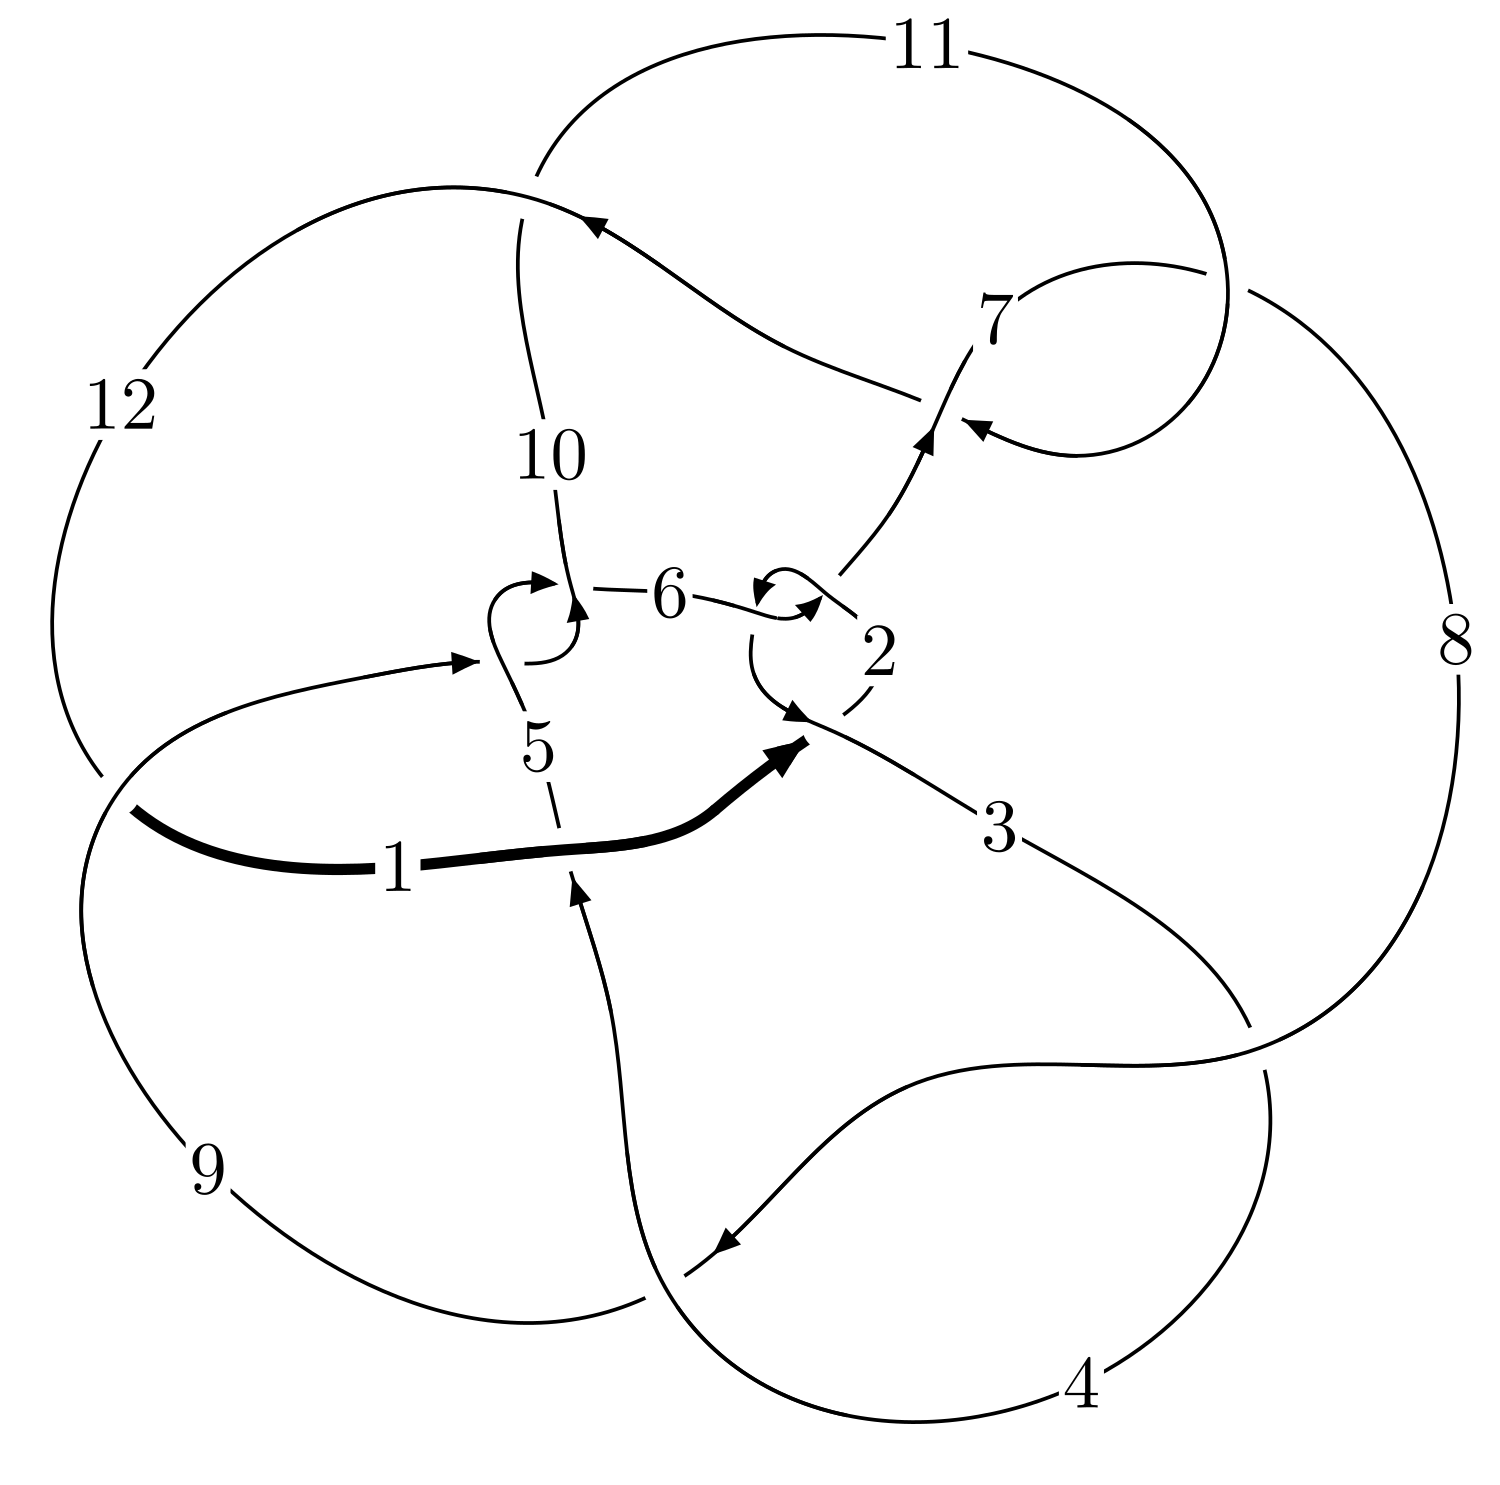
\includegraphics[width=112pt]{../../../GIT/diagram.site/Diagrams/png/1142_12a_0341.png}\\
\ \ \ A knot diagram\footnotemark}&
\allowdisplaybreaks
\textbf{Linearized knot diagam} \\
\cline{2-2}
 &
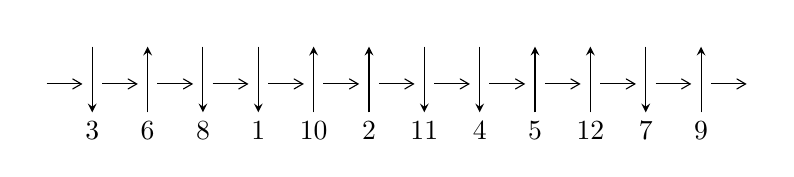
\begin{tikzpicture}[x=20pt, y=17pt]
	% nodes
	\node (C0) at (0, 0) {};
	\node (C1) at (1, 0) {};
	\node (C1U) at (1, +1) {};
	\node (C1D) at (1, -1) {3};

	\node (C2) at (2, 0) {};
	\node (C2U) at (2, +1) {};
	\node (C2D) at (2, -1) {6};

	\node (C3) at (3, 0) {};
	\node (C3U) at (3, +1) {};
	\node (C3D) at (3, -1) {8};

	\node (C4) at (4, 0) {};
	\node (C4U) at (4, +1) {};
	\node (C4D) at (4, -1) {1};

	\node (C5) at (5, 0) {};
	\node (C5U) at (5, +1) {};
	\node (C5D) at (5, -1) {10};

	\node (C6) at (6, 0) {};
	\node (C6U) at (6, +1) {};
	\node (C6D) at (6, -1) {2};

	\node (C7) at (7, 0) {};
	\node (C7U) at (7, +1) {};
	\node (C7D) at (7, -1) {11};

	\node (C8) at (8, 0) {};
	\node (C8U) at (8, +1) {};
	\node (C8D) at (8, -1) {4};

	\node (C9) at (9, 0) {};
	\node (C9U) at (9, +1) {};
	\node (C9D) at (9, -1) {5};

	\node (C10) at (10, 0) {};
	\node (C10U) at (10, +1) {};
	\node (C10D) at (10, -1) {12};

	\node (C11) at (11, 0) {};
	\node (C11U) at (11, +1) {};
	\node (C11D) at (11, -1) {7};

	\node (C12) at (12, 0) {};
	\node (C12U) at (12, +1) {};
	\node (C12D) at (12, -1) {9};
	\node (C13) at (13, 0) {};

	% arrows
	\draw[->,>={angle 60}]
	(C0) edge (C1) (C1) edge (C2) (C2) edge (C3) (C3) edge (C4) (C4) edge (C5) (C5) edge (C6) (C6) edge (C7) (C7) edge (C8) (C8) edge (C9) (C9) edge (C10) (C10) edge (C11) (C11) edge (C12) (C12) edge (C13) ;	\draw[->,>=stealth]
	(C1U) edge (C1D) (C2D) edge (C2U) (C3U) edge (C3D) (C4U) edge (C4D) (C5D) edge (C5U) (C6D) edge (C6U) (C7U) edge (C7D) (C8U) edge (C8D) (C9D) edge (C9U) (C10D) edge (C10U) (C11U) edge (C11D) (C12D) edge (C12U) ;
	\end{tikzpicture} \\
\hhline{~~} \\& 
\textbf{Solving Sequence} \\ \cline{2-2} 
 &
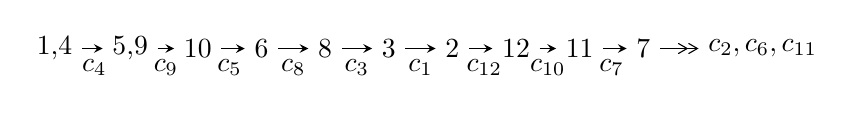
\begin{tikzpicture}[x=23pt, y=7pt]
	% node
	\node (A0) at (-1/8, 0) {1,4};
	\node (A1) at (17/16, 0) {5,9};
	\node (A2) at (17/8, 0) {10};
	\node (A3) at (25/8, 0) {6};
	\node (A4) at (33/8, 0) {8};
	\node (A5) at (41/8, 0) {3};
	\node (A6) at (49/8, 0) {2};
	\node (A7) at (57/8, 0) {12};
	\node (A8) at (65/8, 0) {11};
	\node (A9) at (73/8, 0) {7};
	\node (C1) at (1/2, -1) {$c_{4}$};
	\node (C2) at (13/8, -1) {$c_{9}$};
	\node (C3) at (21/8, -1) {$c_{5}$};
	\node (C4) at (29/8, -1) {$c_{8}$};
	\node (C5) at (37/8, -1) {$c_{3}$};
	\node (C6) at (45/8, -1) {$c_{1}$};
	\node (C7) at (53/8, -1) {$c_{12}$};
	\node (C8) at (61/8, -1) {$c_{10}$};
	\node (C9) at (69/8, -1) {$c_{7}$};
	\node (A10) at (11, 0) {$c_{2},c_{6},c_{11}$};

	% edge
	\draw[->,>=stealth]	
	(A0) edge (A1) (A1) edge (A2) (A2) edge (A3) (A3) edge (A4) (A4) edge (A5) (A5) edge (A6) (A6) edge (A7) (A7) edge (A8) (A8) edge (A9) ;
	\draw[->>,>={angle 60}]	
	(A9) edge (A10);
\end{tikzpicture} \\ 

\end{tabular} \\

\footnotetext{
The image of knot diagram is generated by the software ``\textbf{Draw programme}" developed by Andrew Bartholomew(\url{http://www.layer8.co.uk/maths/draw/index.htm\#Running-draw}), where we modified some parts for our purpose(\url{https://github.com/CATsTAILs/LinksPainter}).
}\phantom \\ \newline 
\centering \textbf{Ideals for irreducible components\footnotemark of $X_{\text{par}}$} 
 
\begin{align*}
I^u_{1}&=\langle 
-3.44332\times10^{1136} u^{137}+2.78439\times10^{1137} u^{136}+\cdots+3.44849\times10^{1135} b-1.92073\times10^{1137},\\
\phantom{I^u_{1}}&\phantom{= \langle  }2.22539\times10^{1128} u^{137}-1.98801\times10^{1129} u^{136}+\cdots+1.86692\times10^{1126} a-8.75584\times10^{1128},\\
\phantom{I^u_{1}}&\phantom{= \langle  }u^{138}-9 u^{137}+\cdots-21 u+1\rangle \\
I^u_{2}&=\langle 
3.23979\times10^{24} u^{23}+6.24896\times10^{24} u^{22}+\cdots+1.91625\times10^{23} b+4.39693\times10^{24},\\
\phantom{I^u_{2}}&\phantom{= \langle  }-2.23743\times10^{23} u^{23}-5.98054\times10^{23} u^{22}+\cdots+3.83250\times10^{22} a-1.44899\times10^{24},\;u^{24}+2 u^{23}+\cdots+8 u+1\rangle \\
\\
\end{align*}
\raggedright * 2 irreducible components of $\dim_{\mathbb{C}}=0$, with total 162 representations.\\
\footnotetext{All coefficients of polynomials are rational numbers. But the coefficients are sometimes approximated in decimal forms when there is not enough margin.}
\newpage
\renewcommand{\arraystretch}{1}
\centering \section*{I. $I^u_{1}= \langle -3.44\times10^{1136} u^{137}+2.78\times10^{1137} u^{136}+\cdots+3.45\times10^{1135} b-1.92\times10^{1137},\;2.23\times10^{1128} u^{137}-1.99\times10^{1129} u^{136}+\cdots+1.87\times10^{1126} a-8.76\times10^{1128},\;u^{138}-9 u^{137}+\cdots-21 u+1 \rangle$}
\flushleft \textbf{(i) Arc colorings}\\
\begin{tabular}{m{7pt} m{180pt} m{7pt} m{180pt} }
\flushright $a_{1}=$&$\begin{pmatrix}0\\u\end{pmatrix}$ \\
\flushright $a_{4}=$&$\begin{pmatrix}1\\0\end{pmatrix}$ \\
\flushright $a_{5}=$&$\begin{pmatrix}1\\u^2\end{pmatrix}$ \\
\flushright $a_{9}=$&$\begin{pmatrix}-119.202 u^{137}+1064.86 u^{136}+\cdots-9035.27 u+469.000\\9.98502 u^{137}-80.7423 u^{136}+\cdots-866.225 u+55.6977\end{pmatrix}$ \\
\flushright $a_{10}=$&$\begin{pmatrix}-116.038 u^{137}+1042.02 u^{136}+\cdots-9853.74 u+516.748\\11.4932 u^{137}-94.3477 u^{136}+\cdots-751.165 u+50.0679\end{pmatrix}$ \\
\flushright $a_{6}=$&$\begin{pmatrix}95.7599 u^{137}-842.835 u^{136}+\cdots+3790.34 u-177.458\\-32.9935 u^{137}+288.022 u^{136}+\cdots-1420.01 u+64.6705\end{pmatrix}$ \\
\flushright $a_{8}=$&$\begin{pmatrix}-109.217 u^{137}+984.122 u^{136}+\cdots-9901.49 u+524.698\\9.98502 u^{137}-80.7423 u^{136}+\cdots-866.225 u+55.6977\end{pmatrix}$ \\
\flushright $a_{3}=$&$\begin{pmatrix}52.6470 u^{137}-472.308 u^{136}+\cdots+3609.65 u-185.644\\-36.0962 u^{137}+312.652 u^{136}+\cdots-1130.23 u+45.1931\end{pmatrix}$ \\
\flushright $a_{2}=$&$\begin{pmatrix}-57.1454 u^{137}+472.524 u^{136}+\cdots+2358.87 u-140.762\\-36.5184 u^{137}+320.362 u^{136}+\cdots-1901.53 u+95.6758\end{pmatrix}$ \\
\flushright $a_{12}=$&$\begin{pmatrix}-30.2955 u^{137}+235.144 u^{136}+\cdots+2935.64 u-137.588\\13.7296 u^{137}-126.491 u^{136}+\cdots+1632.77 u-88.7432\end{pmatrix}$ \\
\flushright $a_{11}=$&$\begin{pmatrix}-118.423 u^{137}+1126.56 u^{136}+\cdots-20434.1 u+1062.67\\-20.6474 u^{137}+188.411 u^{136}+\cdots-2651.47 u+143.008\end{pmatrix}$ \\
\flushright $a_{7}=$&$\begin{pmatrix}28.2171 u^{137}-216.230 u^{136}+\cdots-3099.08 u+146.223\\-18.2326 u^{137}+166.131 u^{136}+\cdots-1907.86 u+102.850\end{pmatrix}$\\&\end{tabular}
\flushleft \textbf{(ii) Obstruction class $= -1$}\\~\\
\flushleft \textbf{(iii) Cusp Shapes $= 113.971 u^{137}-1017.23 u^{136}+\cdots+8375.14 u-424.668$}\\~\\
\newpage\renewcommand{\arraystretch}{1}
\flushleft \textbf{(iv) u-Polynomials at the component}\newline \\
\begin{tabular}{m{50pt}|m{274pt}}
Crossings & \hspace{64pt}u-Polynomials at each crossing \\
\hline $$\begin{aligned}c_{1}\end{aligned}$$&$\begin{aligned}
&u^{138}+61 u^{137}+\cdots+607299 u+14641
\end{aligned}$\\
\hline $$\begin{aligned}c_{2},c_{6}\end{aligned}$$&$\begin{aligned}
&u^{138}- u^{137}+\cdots+1529 u+121
\end{aligned}$\\
\hline $$\begin{aligned}c_{3},c_{8}\end{aligned}$$&$\begin{aligned}
&u^{138}- u^{137}+\cdots-77095 u+4463
\end{aligned}$\\
\hline $$\begin{aligned}c_{4}\end{aligned}$$&$\begin{aligned}
&u^{138}-9 u^{137}+\cdots-21 u+1
\end{aligned}$\\
\hline $$\begin{aligned}c_{5},c_{9}\end{aligned}$$&$\begin{aligned}
&u^{138}+u^{137}+\cdots+77095 u+4463
\end{aligned}$\\
\hline $$\begin{aligned}c_{7},c_{11}\end{aligned}$$&$\begin{aligned}
&u^{138}+u^{137}+\cdots-1529 u+121
\end{aligned}$\\
\hline $$\begin{aligned}c_{10}\end{aligned}$$&$\begin{aligned}
&u^{138}-61 u^{137}+\cdots-607299 u+14641
\end{aligned}$\\
\hline $$\begin{aligned}c_{12}\end{aligned}$$&$\begin{aligned}
&u^{138}+9 u^{137}+\cdots+21 u+1
\end{aligned}$\\
\hline
\end{tabular}\\~\\
\newpage\renewcommand{\arraystretch}{1}
\flushleft \textbf{(v) Riley Polynomials at the component}\newline \\
\begin{tabular}{m{50pt}|m{274pt}}
Crossings & \hspace{64pt}Riley Polynomials at each crossing \\
\hline $$\begin{aligned}c_{1},c_{10}\end{aligned}$$&$\begin{aligned}
&y^{138}+45 y^{137}+\cdots+6338026514699 y+214358881
\end{aligned}$\\
\hline $$\begin{aligned}c_{2},c_{6},c_{7}\\c_{11}\end{aligned}$$&$\begin{aligned}
&y^{138}+61 y^{137}+\cdots+607299 y+14641
\end{aligned}$\\
\hline $$\begin{aligned}c_{3},c_{5},c_{8}\\c_{9}\end{aligned}$$&$\begin{aligned}
&y^{138}-81 y^{137}+\cdots-4595134649 y+19918369
\end{aligned}$\\
\hline $$\begin{aligned}c_{4},c_{12}\end{aligned}$$&$\begin{aligned}
&y^{138}+15 y^{137}+\cdots+45 y+1
\end{aligned}$\\
\hline
\end{tabular}\\~\\
\newpage\flushleft \textbf{(vi) Complex Volumes and Cusp Shapes}
$$\begin{array}{c|c|c}  
\text{Solutions to }I^u_{1}& \I (\text{vol} + \sqrt{-1}CS) & \text{Cusp shape}\\
 \hline 
\begin{aligned}
u &= -0.272105 + 0.972282 I \\
a &= -1.93427 + 1.29974 I \\
b &= \phantom{-}0.992143 - 0.175684 I\end{aligned}
 & \phantom{-}4.46651 + 5.76707 I & \phantom{-0.000000 } 0 \\ \hline\begin{aligned}
u &= -0.272105 - 0.972282 I \\
a &= -1.93427 - 1.29974 I \\
b &= \phantom{-}0.992143 + 0.175684 I\end{aligned}
 & \phantom{-}4.46651 - 5.76707 I & \phantom{-0.000000 } 0 \\ \hline\begin{aligned}
u &= -0.373903 + 0.940772 I \\
a &= -1.02386 + 1.70217 I \\
b &= \phantom{-}0.883629 - 0.470800 I\end{aligned}
 & \phantom{-}3.88225 + 0.20824 I & \phantom{-0.000000 } 0 \\ \hline\begin{aligned}
u &= -0.373903 - 0.940772 I \\
a &= -1.02386 - 1.70217 I \\
b &= \phantom{-}0.883629 + 0.470800 I\end{aligned}
 & \phantom{-}3.88225 - 0.20824 I & \phantom{-0.000000 } 0 \\ \hline\begin{aligned}
u &= \phantom{-}0.752554 + 0.639394 I \\
a &= -0.290394 - 1.355470 I \\
b &= \phantom{-}1.43199 + 0.31863 I\end{aligned}
 & -8.15626 - 5.13625 I & \phantom{-0.000000 } 0 \\ \hline\begin{aligned}
u &= \phantom{-}0.752554 - 0.639394 I \\
a &= -0.290394 + 1.355470 I \\
b &= \phantom{-}1.43199 - 0.31863 I\end{aligned}
 & -8.15626 + 5.13625 I & \phantom{-0.000000 } 0 \\ \hline\begin{aligned}
u &= -0.077192 + 1.013360 I \\
a &= \phantom{-}1.63409 + 0.46381 I \\
b &= -0.553011 - 0.498638 I\end{aligned}
 & \phantom{-}2.01182 + 6.13132 I & \phantom{-0.000000 } 0 \\ \hline\begin{aligned}
u &= -0.077192 - 1.013360 I \\
a &= \phantom{-}1.63409 - 0.46381 I \\
b &= -0.553011 + 0.498638 I\end{aligned}
 & \phantom{-}2.01182 - 6.13132 I & \phantom{-0.000000 } 0 \\ \hline\begin{aligned}
u &= -0.239308 + 0.990831 I \\
a &= \phantom{-}2.06293 - 0.80865 I \\
b &= -0.935928 - 0.016428 I\end{aligned}
 & \phantom{-}3.99322 + 2.29700 I & \phantom{-0.000000 } 0 \\ \hline\begin{aligned}
u &= -0.239308 - 0.990831 I \\
a &= \phantom{-}2.06293 + 0.80865 I \\
b &= -0.935928 + 0.016428 I\end{aligned}
 & \phantom{-}3.99322 - 2.29700 I & \phantom{-0.000000 } 0\\
 \hline 
 \end{array}$$\newpage$$\begin{array}{c|c|c}  
\text{Solutions to }I^u_{1}& \I (\text{vol} + \sqrt{-1}CS) & \text{Cusp shape}\\
 \hline 
\begin{aligned}
u &= \phantom{-}0.060247 + 1.023100 I \\
a &= -1.142720 - 0.824417 I \\
b &= \phantom{-}0.295496 + 0.676979 I\end{aligned}
 & \phantom{-}1.216640 + 0.681103 I & \phantom{-0.000000 } 0 \\ \hline\begin{aligned}
u &= \phantom{-}0.060247 - 1.023100 I \\
a &= -1.142720 + 0.824417 I \\
b &= \phantom{-}0.295496 - 0.676979 I\end{aligned}
 & \phantom{-}1.216640 - 0.681103 I & \phantom{-0.000000 } 0 \\ \hline\begin{aligned}
u &= \phantom{-}0.488193 + 0.911199 I \\
a &= -0.191286 - 1.198690 I \\
b &= -0.093001 + 0.984414 I\end{aligned}
 & \phantom{-}3.67051 - 2.44046 I & \phantom{-0.000000 } 0 \\ \hline\begin{aligned}
u &= \phantom{-}0.488193 - 0.911199 I \\
a &= -0.191286 + 1.198690 I \\
b &= -0.093001 - 0.984414 I\end{aligned}
 & \phantom{-}3.67051 + 2.44046 I & \phantom{-0.000000 } 0 \\ \hline\begin{aligned}
u &= \phantom{-}0.883420 + 0.600790 I \\
a &= \phantom{-}0.190118 + 1.145700 I \\
b &= -1.400590 - 0.186122 I\end{aligned}
 & -8.71911 + 0.66760 I & \phantom{-0.000000 } 0 \\ \hline\begin{aligned}
u &= \phantom{-}0.883420 - 0.600790 I \\
a &= \phantom{-}0.190118 - 1.145700 I \\
b &= -1.400590 + 0.186122 I\end{aligned}
 & -8.71911 - 0.66760 I & \phantom{-0.000000 } 0 \\ \hline\begin{aligned}
u &= -0.664902 + 0.647465 I \\
a &= -0.504665 - 1.102610 I \\
b &= -0.877971 + 0.440649 I\end{aligned}
 & \phantom{-}1.67557 + 2.74433 I & \phantom{-0.000000 } 0 \\ \hline\begin{aligned}
u &= -0.664902 - 0.647465 I \\
a &= -0.504665 + 1.102610 I \\
b &= -0.877971 - 0.440649 I\end{aligned}
 & \phantom{-}1.67557 - 2.74433 I & \phantom{-0.000000 } 0 \\ \hline\begin{aligned}
u &= \phantom{-}0.967854 + 0.469102 I \\
a &= \phantom{-}1.236110 - 0.669379 I \\
b &= \phantom{-}1.042350 + 0.396913 I\end{aligned}
 & -1.11652 - 7.36017 I & \phantom{-0.000000 } 0 \\ \hline\begin{aligned}
u &= \phantom{-}0.967854 - 0.469102 I \\
a &= \phantom{-}1.236110 + 0.669379 I \\
b &= \phantom{-}1.042350 - 0.396913 I\end{aligned}
 & -1.11652 + 7.36017 I & \phantom{-0.000000 } 0\\
 \hline 
 \end{array}$$\newpage$$\begin{array}{c|c|c}  
\text{Solutions to }I^u_{1}& \I (\text{vol} + \sqrt{-1}CS) & \text{Cusp shape}\\
 \hline 
\begin{aligned}
u &= \phantom{-}0.600530 + 0.895121 I \\
a &= \phantom{-}0.011810 + 1.220600 I \\
b &= \phantom{-}0.109514 - 1.079390 I\end{aligned}
 & \phantom{-}6.14091 - 7.61368 I & \phantom{-0.000000 } 0 \\ \hline\begin{aligned}
u &= \phantom{-}0.600530 - 0.895121 I \\
a &= \phantom{-}0.011810 - 1.220600 I \\
b &= \phantom{-}0.109514 + 1.079390 I\end{aligned}
 & \phantom{-}6.14091 + 7.61368 I & \phantom{-0.000000 } 0 \\ \hline\begin{aligned}
u &= \phantom{-}0.912532 + 0.053594 I \\
a &= \phantom{-}0.876109 - 0.975755 I \\
b &= \phantom{-}0.955013 - 0.000219 I\end{aligned}
 & -0.945343 - 0.366206 I & \phantom{-0.000000 } 0 \\ \hline\begin{aligned}
u &= \phantom{-}0.912532 - 0.053594 I \\
a &= \phantom{-}0.876109 + 0.975755 I \\
b &= \phantom{-}0.955013 + 0.000219 I\end{aligned}
 & -0.945343 + 0.366206 I & \phantom{-0.000000 } 0 \\ \hline\begin{aligned}
u &= -1.049450 + 0.406371 I \\
a &= -0.343211 - 0.749855 I \\
b &= -0.0829223 + 0.0313636 I\end{aligned}
 & -1.67557 + 2.74433 I & \phantom{-0.000000 } 0 \\ \hline\begin{aligned}
u &= -1.049450 - 0.406371 I \\
a &= -0.343211 + 0.749855 I \\
b &= -0.0829223 - 0.0313636 I\end{aligned}
 & -1.67557 - 2.74433 I & \phantom{-0.000000 } 0 \\ \hline\begin{aligned}
u &= -0.439694 + 1.049030 I \\
a &= \phantom{-}0.710302 - 1.151910 I \\
b &= -0.661466 + 0.591574 I\end{aligned}
 & \phantom{-}2.23111 + 4.47872 I & \phantom{-0.000000 } 0 \\ \hline\begin{aligned}
u &= -0.439694 - 1.049030 I \\
a &= \phantom{-}0.710302 + 1.151910 I \\
b &= -0.661466 - 0.591574 I\end{aligned}
 & \phantom{-}2.23111 - 4.47872 I & \phantom{-0.000000 } 0 \\ \hline\begin{aligned}
u &= \phantom{-}0.111958 + 0.849954 I \\
a &= \phantom{-}0.535172 - 0.785736 I \\
b &= -0.679053 + 0.478295 I\end{aligned}
 & \phantom{-}2.23634 + 1.17797 I & \phantom{-0.000000 } 0 \\ \hline\begin{aligned}
u &= \phantom{-}0.111958 - 0.849954 I \\
a &= \phantom{-}0.535172 + 0.785736 I \\
b &= -0.679053 - 0.478295 I\end{aligned}
 & \phantom{-}2.23634 - 1.17797 I & \phantom{-0.000000 } 0\\
 \hline 
 \end{array}$$\newpage$$\begin{array}{c|c|c}  
\text{Solutions to }I^u_{1}& \I (\text{vol} + \sqrt{-1}CS) & \text{Cusp shape}\\
 \hline 
\begin{aligned}
u &= \phantom{-}0.938248 + 0.680040 I \\
a &= -0.77268 + 1.39820 I \\
b &= -1.167130 - 0.459804 I\end{aligned}
 & -2.08901 - 4.73737 I & \phantom{-0.000000 } 0 \\ \hline\begin{aligned}
u &= \phantom{-}0.938248 - 0.680040 I \\
a &= -0.77268 - 1.39820 I \\
b &= -1.167130 + 0.459804 I\end{aligned}
 & -2.08901 + 4.73737 I & \phantom{-0.000000 } 0 \\ \hline\begin{aligned}
u &= -0.727757 + 0.366902 I \\
a &= \phantom{-}0.592142 - 0.869379 I \\
b &= \phantom{-}0.448681 - 0.181342 I\end{aligned}
 & -2.23634 + 1.17797 I & \phantom{-0.000000 } 0 \\ \hline\begin{aligned}
u &= -0.727757 - 0.366902 I \\
a &= \phantom{-}0.592142 + 0.869379 I \\
b &= \phantom{-}0.448681 + 0.181342 I\end{aligned}
 & -2.23634 - 1.17797 I & \phantom{-0.000000 } 0 \\ \hline\begin{aligned}
u &= -0.727682 + 0.942031 I \\
a &= -0.573229 - 0.196405 I \\
b &= \phantom{-}0.480323 + 0.508966 I\end{aligned}
 & \phantom{-}0.55047 + 3.64176 I & \phantom{-0.000000 } 0 \\ \hline\begin{aligned}
u &= -0.727682 - 0.942031 I \\
a &= -0.573229 + 0.196405 I \\
b &= \phantom{-}0.480323 - 0.508966 I\end{aligned}
 & \phantom{-}0.55047 - 3.64176 I & \phantom{-0.000000 } 0 \\ \hline\begin{aligned}
u &= -0.851773 + 0.843453 I \\
a &= \phantom{-}0.509465 + 0.567410 I \\
b &= -0.132538 - 0.723809 I\end{aligned}
 & \phantom{-}0.945343 + 0.366206 I & \phantom{-0.000000 } 0 \\ \hline\begin{aligned}
u &= -0.851773 - 0.843453 I \\
a &= \phantom{-}0.509465 - 0.567410 I \\
b &= -0.132538 + 0.723809 I\end{aligned}
 & \phantom{-}0.945343 - 0.366206 I & \phantom{-0.000000 } 0 \\ \hline\begin{aligned}
u &= -0.593004 + 1.056020 I \\
a &= \phantom{-}0.180572 - 1.042790 I \\
b &= -0.139227 + 1.159900 I\end{aligned}
 & \phantom{-}2.42938 + 7.47182 I & \phantom{-0.000000 } 0 \\ \hline\begin{aligned}
u &= -0.593004 - 1.056020 I \\
a &= \phantom{-}0.180572 + 1.042790 I \\
b &= -0.139227 - 1.159900 I\end{aligned}
 & \phantom{-}2.42938 - 7.47182 I & \phantom{-0.000000 } 0\\
 \hline 
 \end{array}$$\newpage$$\begin{array}{c|c|c}  
\text{Solutions to }I^u_{1}& \I (\text{vol} + \sqrt{-1}CS) & \text{Cusp shape}\\
 \hline 
\begin{aligned}
u &= -0.641815 + 1.029010 I \\
a &= -0.050692 + 1.059620 I \\
b &= \phantom{-}0.000038 - 1.294560 I\end{aligned}
 & \phantom{-}4.39065 + 13.04350 I & \phantom{-0.000000 } 0 \\ \hline\begin{aligned}
u &= -0.641815 - 1.029010 I \\
a &= -0.050692 - 1.059620 I \\
b &= \phantom{-}0.000038 + 1.294560 I\end{aligned}
 & \phantom{-}4.39065 - 13.04350 I & \phantom{-0.000000 } 0 \\ \hline\begin{aligned}
u &= -1.132200 + 0.448698 I \\
a &= \phantom{-}0.067608 + 0.361482 I \\
b &= \phantom{-}1.073610 - 0.102452 I\end{aligned}
 & -2.16239 + 0.31280 I & \phantom{-0.000000 } 0 \\ \hline\begin{aligned}
u &= -1.132200 - 0.448698 I \\
a &= \phantom{-}0.067608 - 0.361482 I \\
b &= \phantom{-}1.073610 + 0.102452 I\end{aligned}
 & -2.16239 - 0.31280 I & \phantom{-0.000000 } 0 \\ \hline\begin{aligned}
u &= \phantom{-}0.520373 + 1.126360 I \\
a &= \phantom{-}0.140955 + 0.849436 I \\
b &= \phantom{-}0.264174 - 0.868535 I\end{aligned}
 & \phantom{-}8.71911 + 0.66760 I & \phantom{-0.000000 } 0 \\ \hline\begin{aligned}
u &= \phantom{-}0.520373 - 1.126360 I \\
a &= \phantom{-}0.140955 - 0.849436 I \\
b &= \phantom{-}0.264174 + 0.868535 I\end{aligned}
 & \phantom{-}8.71911 - 0.66760 I & \phantom{-0.000000 } 0 \\ \hline\begin{aligned}
u &= -0.998861 + 0.759491 I \\
a &= -0.129822 + 0.813527 I \\
b &= \phantom{-}1.272690 - 0.445031 I\end{aligned}
 & -3.67051 + 2.44046 I & \phantom{-0.000000 } 0 \\ \hline\begin{aligned}
u &= -0.998861 - 0.759491 I \\
a &= -0.129822 - 0.813527 I \\
b &= \phantom{-}1.272690 + 0.445031 I\end{aligned}
 & -3.67051 - 2.44046 I & \phantom{-0.000000 } 0 \\ \hline\begin{aligned}
u &= -0.291302 + 0.679963 I \\
a &= -0.051473 + 0.427774 I \\
b &= \phantom{-}0.291428 - 0.679082 I\end{aligned}
 & -0.05605 + 1.78094 I & \phantom{-0.000000 } 0 \\ \hline\begin{aligned}
u &= -0.291302 - 0.679963 I \\
a &= -0.051473 - 0.427774 I \\
b &= \phantom{-}0.291428 + 0.679082 I\end{aligned}
 & -0.05605 - 1.78094 I & \phantom{-0.000000 } 0\\
 \hline 
 \end{array}$$\newpage$$\begin{array}{c|c|c}  
\text{Solutions to }I^u_{1}& \I (\text{vol} + \sqrt{-1}CS) & \text{Cusp shape}\\
 \hline 
\begin{aligned}
u &= \phantom{-}1.086430 + 0.662833 I \\
a &= \phantom{-}0.299139 - 0.999413 I \\
b &= \phantom{-}1.128700 + 0.551194 I\end{aligned}
 & -0.74320 - 6.11734 I & \phantom{-0.000000 } 0 \\ \hline\begin{aligned}
u &= \phantom{-}1.086430 - 0.662833 I \\
a &= \phantom{-}0.299139 + 0.999413 I \\
b &= \phantom{-}1.128700 - 0.551194 I\end{aligned}
 & -0.74320 + 6.11734 I & \phantom{-0.000000 } 0 \\ \hline\begin{aligned}
u &= -0.602148 + 0.397079 I \\
a &= -1.56122 + 0.53492 I \\
b &= -0.544434 + 0.347223 I\end{aligned}
 & -0.55047 - 3.64176 I & \phantom{-0.000000 } 0 \\ \hline\begin{aligned}
u &= -0.602148 - 0.397079 I \\
a &= -1.56122 - 0.53492 I \\
b &= -0.544434 - 0.347223 I\end{aligned}
 & -0.55047 + 3.64176 I & \phantom{-0.000000 } 0 \\ \hline\begin{aligned}
u &= -0.994126 + 0.809066 I \\
a &= \phantom{-}0.161223 - 0.931048 I \\
b &= -1.30468 + 0.58986 I\end{aligned}
 & -2.42938 + 7.47182 I & \phantom{-0.000000 } 0 \\ \hline\begin{aligned}
u &= -0.994126 - 0.809066 I \\
a &= \phantom{-}0.161223 + 0.931048 I \\
b &= -1.30468 - 0.58986 I\end{aligned}
 & -2.42938 - 7.47182 I & \phantom{-0.000000 } 0 \\ \hline\begin{aligned}
u &= \phantom{-}1.057830 + 0.732243 I \\
a &= -0.045045 - 0.941580 I \\
b &= \phantom{-}1.43238 + 0.67601 I\end{aligned}
 & -4.39065 - 13.04350 I & \phantom{-0.000000 } 0 \\ \hline\begin{aligned}
u &= \phantom{-}1.057830 - 0.732243 I \\
a &= -0.045045 + 0.941580 I \\
b &= \phantom{-}1.43238 - 0.67601 I\end{aligned}
 & -4.39065 + 13.04350 I & \phantom{-0.000000 } 0 \\ \hline\begin{aligned}
u &= -0.698312 + 0.116861 I \\
a &= \phantom{-}0.273726 + 0.345184 I \\
b &= -1.181700 - 0.509825 I\end{aligned}
 & \phantom{-}1.11025 + 3.10329 I & \phantom{-0.000000 } 0 \\ \hline\begin{aligned}
u &= -0.698312 - 0.116861 I \\
a &= \phantom{-}0.273726 - 0.345184 I \\
b &= -1.181700 + 0.509825 I\end{aligned}
 & \phantom{-}1.11025 - 3.10329 I & \phantom{-0.000000 } 0\\
 \hline 
 \end{array}$$\newpage$$\begin{array}{c|c|c}  
\text{Solutions to }I^u_{1}& \I (\text{vol} + \sqrt{-1}CS) & \text{Cusp shape}\\
 \hline 
\begin{aligned}
u &= \phantom{-}0.951156 + 0.881801 I \\
a &= -0.05261 + 1.52270 I \\
b &= -1.314470 - 0.312706 I\end{aligned}
 & -4.75617 - 9.62715 I & \phantom{-0.000000 } 0 \\ \hline\begin{aligned}
u &= \phantom{-}0.951156 - 0.881801 I \\
a &= -0.05261 - 1.52270 I \\
b &= -1.314470 + 0.312706 I\end{aligned}
 & -4.75617 + 9.62715 I & \phantom{-0.000000 } 0 \\ \hline\begin{aligned}
u &= \phantom{-}1.085490 + 0.743576 I \\
a &= \phantom{-}0.007926 + 0.819196 I \\
b &= -1.42697 - 0.55428 I\end{aligned}
 & -6.14091 - 7.61368 I & \phantom{-0.000000 } 0 \\ \hline\begin{aligned}
u &= \phantom{-}1.085490 - 0.743576 I \\
a &= \phantom{-}0.007926 - 0.819196 I \\
b &= -1.42697 + 0.55428 I\end{aligned}
 & -6.14091 + 7.61368 I & \phantom{-0.000000 } 0 \\ \hline\begin{aligned}
u &= -0.971836 + 0.903292 I \\
a &= -0.073011 - 0.997331 I \\
b &= -0.880200 + 0.799810 I\end{aligned}
 & \phantom{-0.000000 -}2.77105 I & \phantom{-0.000000 } 0 \\ \hline\begin{aligned}
u &= -0.971836 - 0.903292 I \\
a &= -0.073011 + 0.997331 I \\
b &= -0.880200 - 0.799810 I\end{aligned}
 & \phantom{-0.000000 } -2.77105 I & \phantom{-0.000000 } 0 \\ \hline\begin{aligned}
u &= -0.987437 + 0.887515 I \\
a &= \phantom{-}0.274865 + 0.918316 I \\
b &= \phantom{-}0.532355 - 0.860913 I\end{aligned}
 & \phantom{-}0.74320 + 6.11734 I & \phantom{-0.000000 } 0 \\ \hline\begin{aligned}
u &= -0.987437 - 0.887515 I \\
a &= \phantom{-}0.274865 - 0.918316 I \\
b &= \phantom{-}0.532355 + 0.860913 I\end{aligned}
 & \phantom{-}0.74320 - 6.11734 I & \phantom{-0.000000 } 0 \\ \hline\begin{aligned}
u &= -0.648145 + 1.205740 I \\
a &= -0.151118 + 0.705374 I \\
b &= -0.173279 - 0.811593 I\end{aligned}
 & \phantom{-}8.15626 + 5.13625 I & \phantom{-0.000000 } 0 \\ \hline\begin{aligned}
u &= -0.648145 - 1.205740 I \\
a &= -0.151118 - 0.705374 I \\
b &= -0.173279 + 0.811593 I\end{aligned}
 & \phantom{-}8.15626 - 5.13625 I & \phantom{-0.000000 } 0\\
 \hline 
 \end{array}$$\newpage$$\begin{array}{c|c|c}  
\text{Solutions to }I^u_{1}& \I (\text{vol} + \sqrt{-1}CS) & \text{Cusp shape}\\
 \hline 
\begin{aligned}
u &= \phantom{-}1.024050 + 0.930465 I \\
a &= -0.028357 - 1.275540 I \\
b &= \phantom{-}1.260970 + 0.226165 I\end{aligned}
 & -5.93710 - 4.34590 I & \phantom{-0.000000 } 0 \\ \hline\begin{aligned}
u &= \phantom{-}1.024050 - 0.930465 I \\
a &= -0.028357 + 1.275540 I \\
b &= \phantom{-}1.260970 - 0.226165 I\end{aligned}
 & -5.93710 + 4.34590 I & \phantom{-0.000000 } 0 \\ \hline\begin{aligned}
u &= \phantom{-}0.436460 + 0.425557 I \\
a &= -1.60395 + 1.88000 I \\
b &= \phantom{-}0.456253 - 0.433194 I\end{aligned}
 & \phantom{-}4.93848 + 3.64554 I & \phantom{-0.000000 } 0 \\ \hline\begin{aligned}
u &= \phantom{-}0.436460 - 0.425557 I \\
a &= -1.60395 - 1.88000 I \\
b &= \phantom{-}0.456253 + 0.433194 I\end{aligned}
 & \phantom{-}4.93848 - 3.64554 I & \phantom{-0.000000 } 0 \\ \hline\begin{aligned}
u &= -0.77462 + 1.21878 I \\
a &= -0.575541 + 0.415227 I \\
b &= \phantom{-}0.998111 + 0.042104 I\end{aligned}
 & -1.216640 - 0.681103 I & \phantom{-0.000000 } 0 \\ \hline\begin{aligned}
u &= -0.77462 - 1.21878 I \\
a &= -0.575541 - 0.415227 I \\
b &= \phantom{-}0.998111 - 0.042104 I\end{aligned}
 & -1.216640 + 0.681103 I & \phantom{-0.000000 } 0 \\ \hline\begin{aligned}
u &= \phantom{-}0.194293 + 0.483947 I \\
a &= -0.204689 + 0.649331 I \\
b &= \phantom{-}1.09528 - 1.37945 I\end{aligned}
 & -0.444360 + 0.758531 I & \phantom{-}14.6583 + 7.5400 I \\ \hline\begin{aligned}
u &= \phantom{-}0.194293 - 0.483947 I \\
a &= -0.204689 - 0.649331 I \\
b &= \phantom{-}1.09528 + 1.37945 I\end{aligned}
 & -0.444360 - 0.758531 I & \phantom{-}14.6583 - 7.5400 I \\ \hline\begin{aligned}
u &= \phantom{-}1.50011 + 0.13797 I \\
a &= -0.262639 + 0.307841 I \\
b &= -1.169710 + 0.144965 I\end{aligned}
 & -4.93848 + 3.64554 I & \phantom{-0.000000 } 0 \\ \hline\begin{aligned}
u &= \phantom{-}1.50011 - 0.13797 I \\
a &= -0.262639 - 0.307841 I \\
b &= -1.169710 - 0.144965 I\end{aligned}
 & -4.93848 - 3.64554 I & \phantom{-0.000000 } 0\\
 \hline 
 \end{array}$$\newpage$$\begin{array}{c|c|c}  
\text{Solutions to }I^u_{1}& \I (\text{vol} + \sqrt{-1}CS) & \text{Cusp shape}\\
 \hline 
\begin{aligned}
u &= -0.486377 + 0.050195 I \\
a &= -0.227084 - 0.673388 I \\
b &= \phantom{-}1.17421 + 1.25375 I\end{aligned}
 & \phantom{-}0.846297 + 0.024641 I & -15.5429 - 7.8844 I \\ \hline\begin{aligned}
u &= -0.486377 - 0.050195 I \\
a &= -0.227084 + 0.673388 I \\
b &= \phantom{-}1.17421 - 1.25375 I\end{aligned}
 & \phantom{-}0.846297 - 0.024641 I & -15.5429 + 7.8844 I \\ \hline\begin{aligned}
u &= -1.51038 + 0.06800 I \\
a &= \phantom{-}0.625551 + 0.338750 I \\
b &= \phantom{-}0.451371 + 0.245792 I\end{aligned}
 & \phantom{-}1.11652 + 7.36017 I & \phantom{-0.000000 } 0 \\ \hline\begin{aligned}
u &= -1.51038 - 0.06800 I \\
a &= \phantom{-}0.625551 - 0.338750 I \\
b &= \phantom{-}0.451371 - 0.245792 I\end{aligned}
 & \phantom{-}1.11652 - 7.36017 I & \phantom{-0.000000 } 0 \\ \hline\begin{aligned}
u &= -0.89607 + 1.25161 I \\
a &= \phantom{-}0.387843 - 0.628970 I \\
b &= -1.045510 + 0.201901 I\end{aligned}
 & -2.23111 + 4.47872 I & \phantom{-0.000000 } 0 \\ \hline\begin{aligned}
u &= -0.89607 - 1.25161 I \\
a &= \phantom{-}0.387843 + 0.628970 I \\
b &= -1.045510 - 0.201901 I\end{aligned}
 & -2.23111 - 4.47872 I & \phantom{-0.000000 } 0 \\ \hline\begin{aligned}
u &= \phantom{-}0.238742 + 0.378933 I \\
a &= \phantom{-}0.49991 - 2.67289 I \\
b &= -0.633279 + 0.424355 I\end{aligned}
 & \phantom{-}2.16239 - 0.31280 I & \phantom{-}3.87060 + 0. I\phantom{ +0.000000I} \\ \hline\begin{aligned}
u &= \phantom{-}0.238742 - 0.378933 I \\
a &= \phantom{-}0.49991 + 2.67289 I \\
b &= -0.633279 - 0.424355 I\end{aligned}
 & \phantom{-}2.16239 + 0.31280 I & \phantom{-}3.87060 + 0. I\phantom{ +0.000000I} \\ \hline\begin{aligned}
u &= -1.02413 + 1.19332 I \\
a &= -0.156612 + 1.088080 I \\
b &= \phantom{-}1.30906 - 0.55402 I\end{aligned}
 & \phantom{-}2.37368 + 13.37220 I & \phantom{-0.000000 } 0 \\ \hline\begin{aligned}
u &= -1.02413 - 1.19332 I \\
a &= -0.156612 - 1.088080 I \\
b &= \phantom{-}1.30906 + 0.55402 I\end{aligned}
 & \phantom{-}2.37368 - 13.37220 I & \phantom{-0.000000 } 0\\
 \hline 
 \end{array}$$\newpage$$\begin{array}{c|c|c}  
\text{Solutions to }I^u_{1}& \I (\text{vol} + \sqrt{-1}CS) & \text{Cusp shape}\\
 \hline 
\begin{aligned}
u &= -1.00813 + 1.23712 I \\
a &= \phantom{-}0.201878 - 0.979411 I \\
b &= -1.273390 + 0.502557 I\end{aligned}
 & \phantom{-0.000000 -}7.71222 I & \phantom{-0.000000 } 0 \\ \hline\begin{aligned}
u &= -1.00813 - 1.23712 I \\
a &= \phantom{-}0.201878 + 0.979411 I \\
b &= -1.273390 - 0.502557 I\end{aligned}
 & \phantom{-0.000000 } -7.71222 I & \phantom{-0.000000 } 0 \\ \hline\begin{aligned}
u &= \phantom{-}0.277315 + 0.283202 I \\
a &= \phantom{-}0.104752 - 0.888653 I \\
b &= -1.22541 + 1.68513 I\end{aligned}
 & \phantom{-}0.31243 + 4.65765 I & -0.5140 + 24.9918 I \\ \hline\begin{aligned}
u &= \phantom{-}0.277315 - 0.283202 I \\
a &= \phantom{-}0.104752 + 0.888653 I \\
b &= -1.22541 - 1.68513 I\end{aligned}
 & \phantom{-}0.31243 - 4.65765 I & -0.5140 - 24.9918 I \\ \hline\begin{aligned}
u &= \phantom{-}0.354011 + 0.027102 I \\
a &= -0.44159 + 1.40084 I \\
b &= -1.17718 - 1.21340 I\end{aligned}
 & \phantom{-}0.444360 + 0.758531 I & -14.6583 + 7.5400 I \\ \hline\begin{aligned}
u &= \phantom{-}0.354011 - 0.027102 I \\
a &= -0.44159 - 1.40084 I \\
b &= -1.17718 + 1.21340 I\end{aligned}
 & \phantom{-}0.444360 - 0.758531 I & -14.6583 - 7.5400 I \\ \hline\begin{aligned}
u &= -0.280718 + 0.216771 I \\
a &= \phantom{-}0.130829 + 1.109880 I \\
b &= \phantom{-}1.36464 - 1.66574 I\end{aligned}
 & -0.31243 - 4.65765 I & \phantom{-}0.5140 - 24.9918 I \\ \hline\begin{aligned}
u &= -0.280718 - 0.216771 I \\
a &= \phantom{-}0.130829 - 1.109880 I \\
b &= \phantom{-}1.36464 + 1.66574 I\end{aligned}
 & -0.31243 + 4.65765 I & \phantom{-}0.5140 + 24.9918 I \\ \hline\begin{aligned}
u &= -0.144249 + 0.316122 I \\
a &= -0.449654 - 1.333390 I \\
b &= -1.26024 + 1.40027 I\end{aligned}
 & -0.846297 + 0.024641 I & \phantom{-}15.5429 - 7.8844 I \\ \hline\begin{aligned}
u &= -0.144249 - 0.316122 I \\
a &= -0.449654 + 1.333390 I \\
b &= -1.26024 - 1.40027 I\end{aligned}
 & -0.846297 - 0.024641 I & \phantom{-}15.5429 + 7.8844 I\\
 \hline 
 \end{array}$$\newpage$$\begin{array}{c|c|c}  
\text{Solutions to }I^u_{1}& \I (\text{vol} + \sqrt{-1}CS) & \text{Cusp shape}\\
 \hline 
\begin{aligned}
u &= \phantom{-}0.249069 + 0.221274 I \\
a &= -1.43089 + 5.48760 I \\
b &= \phantom{-}0.666087 - 0.201597 I\end{aligned}
 & \phantom{-}5.28142 - 3.87461 I & \phantom{-}7.78917 + 1.22770 I \\ \hline\begin{aligned}
u &= \phantom{-}0.249069 - 0.221274 I \\
a &= -1.43089 - 5.48760 I \\
b &= \phantom{-}0.666087 + 0.201597 I\end{aligned}
 & \phantom{-}5.28142 + 3.87461 I & \phantom{-}7.78917 - 1.22770 I \\ \hline\begin{aligned}
u &= \phantom{-}1.13993 + 1.22922 I \\
a &= \phantom{-}0.075276 + 0.997163 I \\
b &= -1.40521 - 0.60727 I\end{aligned}
 & \phantom{-0.000000 } -19.6086 I & \phantom{-0.000000 } 0 \\ \hline\begin{aligned}
u &= \phantom{-}1.13993 - 1.22922 I \\
a &= \phantom{-}0.075276 - 0.997163 I \\
b &= -1.40521 + 0.60727 I\end{aligned}
 & \phantom{-0.000000 -}19.6086 I & \phantom{-0.000000 } 0 \\ \hline\begin{aligned}
u &= \phantom{-}0.275876 + 0.159611 I \\
a &= -0.27727 - 2.30432 I \\
b &= -0.102535 + 0.537992 I\end{aligned}
 & \phantom{-}0.05605 - 1.78094 I & -0.01856 + 2.95154 I \\ \hline\begin{aligned}
u &= \phantom{-}0.275876 - 0.159611 I \\
a &= -0.27727 + 2.30432 I \\
b &= -0.102535 - 0.537992 I\end{aligned}
 & \phantom{-}0.05605 + 1.78094 I & -0.01856 - 2.95154 I \\ \hline\begin{aligned}
u &= \phantom{-}0.231485 + 0.209058 I \\
a &= \phantom{-}1.41039 - 1.77858 I \\
b &= \phantom{-}1.36778 + 0.62876 I\end{aligned}
 & -1.11025 - 3.10329 I & \phantom{-}2.30522 + 6.70707 I \\ \hline\begin{aligned}
u &= \phantom{-}0.231485 - 0.209058 I \\
a &= \phantom{-}1.41039 + 1.77858 I \\
b &= \phantom{-}1.36778 - 0.62876 I\end{aligned}
 & -1.11025 + 3.10329 I & \phantom{-}2.30522 - 6.70707 I \\ \hline\begin{aligned}
u &= \phantom{-}0.099745 + 0.272426 I \\
a &= \phantom{-}4.23217 - 4.46581 I \\
b &= \phantom{-}1.053940 + 0.392703 I\end{aligned}
 & -0.95266 - 4.76806 I & \phantom{-}0.06588 + 5.12711 I \\ \hline\begin{aligned}
u &= \phantom{-}0.099745 - 0.272426 I \\
a &= \phantom{-}4.23217 + 4.46581 I \\
b &= \phantom{-}1.053940 - 0.392703 I\end{aligned}
 & -0.95266 + 4.76806 I & \phantom{-}0.06588 - 5.12711 I\\
 \hline 
 \end{array}$$\newpage$$\begin{array}{c|c|c}  
\text{Solutions to }I^u_{1}& \I (\text{vol} + \sqrt{-1}CS) & \text{Cusp shape}\\
 \hline 
\begin{aligned}
u &= \phantom{-}0.66367 + 1.58003 I \\
a &= -0.143463 + 0.008026 I \\
b &= \phantom{-}1.299960 - 0.196269 I\end{aligned}
 & -3.43891 + 2.81616 I & \phantom{-0.000000 } 0 \\ \hline\begin{aligned}
u &= \phantom{-}0.66367 - 1.58003 I \\
a &= -0.143463 - 0.008026 I \\
b &= \phantom{-}1.299960 + 0.196269 I\end{aligned}
 & -3.43891 - 2.81616 I & \phantom{-0.000000 } 0 \\ \hline\begin{aligned}
u &= \phantom{-}0.59614 + 1.62012 I \\
a &= \phantom{-}0.566338 + 0.160746 I \\
b &= -1.042740 + 0.230532 I\end{aligned}
 & -2.01182 + 6.13132 I & \phantom{-0.000000 } 0 \\ \hline\begin{aligned}
u &= \phantom{-}0.59614 - 1.62012 I \\
a &= \phantom{-}0.566338 - 0.160746 I \\
b &= -1.042740 - 0.230532 I\end{aligned}
 & -2.01182 - 6.13132 I & \phantom{-0.000000 } 0 \\ \hline\begin{aligned}
u &= \phantom{-}1.13804 + 1.30123 I \\
a &= -0.129597 - 0.900394 I \\
b &= \phantom{-}1.40922 + 0.52861 I\end{aligned}
 & -2.37368 - 13.37220 I & \phantom{-0.000000 } 0 \\ \hline\begin{aligned}
u &= \phantom{-}1.13804 - 1.30123 I \\
a &= -0.129597 + 0.900394 I \\
b &= \phantom{-}1.40922 - 0.52861 I\end{aligned}
 & -2.37368 + 13.37220 I & \phantom{-0.000000 } 0 \\ \hline\begin{aligned}
u &= \phantom{-}0.066659 + 0.257288 I \\
a &= -6.18103 + 6.58510 I \\
b &= -0.947872 - 0.366307 I\end{aligned}
 & \phantom{-}0.93987 - 9.73689 I & \phantom{-}3.92710 + 12.05743 I \\ \hline\begin{aligned}
u &= \phantom{-}0.066659 - 0.257288 I \\
a &= -6.18103 - 6.58510 I \\
b &= -0.947872 + 0.366307 I\end{aligned}
 & \phantom{-}0.93987 + 9.73689 I & \phantom{-}3.92710 - 12.05743 I \\ \hline\begin{aligned}
u &= \phantom{-}0.107893 + 0.221349 I \\
a &= -6.94870 - 0.38873 I \\
b &= -1.021830 - 0.121107 I\end{aligned}
 & \phantom{-}3.43891 - 2.81616 I & \phantom{-}2.08219 + 3.38759 I \\ \hline\begin{aligned}
u &= \phantom{-}0.107893 - 0.221349 I \\
a &= -6.94870 + 0.38873 I \\
b &= -1.021830 + 0.121107 I\end{aligned}
 & \phantom{-}3.43891 + 2.81616 I & \phantom{-}2.08219 - 3.38759 I\\
 \hline 
 \end{array}$$\newpage$$\begin{array}{c|c|c}  
\text{Solutions to }I^u_{1}& \I (\text{vol} + \sqrt{-1}CS) & \text{Cusp shape}\\
 \hline 
\begin{aligned}
u &= -1.15781 + 1.33260 I \\
a &= -0.017420 + 0.783594 I \\
b &= \phantom{-}1.164610 - 0.513507 I\end{aligned}
 & \phantom{-}5.93710 + 4.34590 I & \phantom{-0.000000 } 0 \\ \hline\begin{aligned}
u &= -1.15781 - 1.33260 I \\
a &= -0.017420 - 0.783594 I \\
b &= \phantom{-}1.164610 + 0.513507 I\end{aligned}
 & \phantom{-}5.93710 - 4.34590 I & \phantom{-0.000000 } 0 \\ \hline\begin{aligned}
u &= -1.63874 + 0.70751 I \\
a &= \phantom{-}0.111800 - 0.117972 I \\
b &= -1.083230 - 0.124303 I\end{aligned}
 & \phantom{-}0.95266 - 4.76806 I & \phantom{-0.000000 } 0 \\ \hline\begin{aligned}
u &= -1.63874 - 0.70751 I \\
a &= \phantom{-}0.111800 + 0.117972 I \\
b &= -1.083230 + 0.124303 I\end{aligned}
 & \phantom{-}0.95266 + 4.76806 I & \phantom{-0.000000 } 0 \\ \hline\begin{aligned}
u &= \phantom{-}1.67580 + 0.78640 I \\
a &= -0.302776 + 0.547884 I \\
b &= -0.939973 - 0.058035 I\end{aligned}
 & \phantom{-}2.08901 - 4.73737 I & \phantom{-0.000000 } 0 \\ \hline\begin{aligned}
u &= \phantom{-}1.67580 - 0.78640 I \\
a &= -0.302776 - 0.547884 I \\
b &= -0.939973 + 0.058035 I\end{aligned}
 & \phantom{-}2.08901 + 4.73737 I & \phantom{-0.000000 } 0 \\ \hline\begin{aligned}
u &= \phantom{-}1.57066 + 1.05017 I \\
a &= -0.044491 + 0.170628 I \\
b &= -1.289670 - 0.115617 I\end{aligned}
 & -5.28142 - 3.87461 I & \phantom{-0.000000 } 0 \\ \hline\begin{aligned}
u &= \phantom{-}1.57066 - 1.05017 I \\
a &= -0.044491 - 0.170628 I \\
b &= -1.289670 + 0.115617 I\end{aligned}
 & -5.28142 + 3.87461 I & \phantom{-0.000000 } 0 \\ \hline\begin{aligned}
u &= \phantom{-}1.39276 + 1.40193 I \\
a &= -0.022664 + 0.655944 I \\
b &= -1.246490 - 0.418023 I\end{aligned}
 & \phantom{-}4.75617 - 9.62715 I & \phantom{-0.000000 } 0 \\ \hline\begin{aligned}
u &= \phantom{-}1.39276 - 1.40193 I \\
a &= -0.022664 - 0.655944 I \\
b &= -1.246490 + 0.418023 I\end{aligned}
 & \phantom{-}4.75617 + 9.62715 I & \phantom{-0.000000 } 0\\
 \hline 
 \end{array}$$\newpage$$\begin{array}{c|c|c}  
\text{Solutions to }I^u_{1}& \I (\text{vol} + \sqrt{-1}CS) & \text{Cusp shape}\\
 \hline 
\begin{aligned}
u &= \phantom{-}1.21853 + 1.59967 I \\
a &= -0.259489 - 0.431401 I \\
b &= \phantom{-}1.076910 - 0.077439 I\end{aligned}
 & -3.88225 - 0.20824 I & \phantom{-0.000000 } 0 \\ \hline\begin{aligned}
u &= \phantom{-}1.21853 - 1.59967 I \\
a &= -0.259489 + 0.431401 I \\
b &= \phantom{-}1.076910 + 0.077439 I\end{aligned}
 & -3.88225 + 0.20824 I & \phantom{-0.000000 } 0 \\ \hline\begin{aligned}
u &= -0.30756 + 2.23753 I \\
a &= \phantom{-}0.420183 - 0.164709 I \\
b &= -1.354690 + 0.214286 I\end{aligned}
 & -3.99322 + 2.29700 I & \phantom{-0.000000 } 0 \\ \hline\begin{aligned}
u &= -0.30756 - 2.23753 I \\
a &= \phantom{-}0.420183 + 0.164709 I \\
b &= -1.354690 - 0.214286 I\end{aligned}
 & -3.99322 - 2.29700 I & \phantom{-0.000000 } 0 \\ \hline\begin{aligned}
u &= \phantom{-}0.73739 + 2.23432 I \\
a &= -0.356171 - 0.239331 I \\
b &= \phantom{-}1.380890 + 0.066703 I\end{aligned}
 & -4.46651 - 5.76707 I & \phantom{-0.000000 } 0 \\ \hline\begin{aligned}
u &= \phantom{-}0.73739 - 2.23432 I \\
a &= -0.356171 + 0.239331 I \\
b &= \phantom{-}1.380890 - 0.066703 I\end{aligned}
 & -4.46651 + 5.76707 I & \phantom{-0.000000 } 0 \\ \hline\begin{aligned}
u &= \phantom{-}2.10629 + 1.15135 I \\
a &= -0.0757770 - 0.0807308 I \\
b &= \phantom{-}1.103700 - 0.252363 I\end{aligned}
 & -0.93987 + 9.73689 I & \phantom{-0.000000 } 0 \\ \hline\begin{aligned}
u &= \phantom{-}2.10629 - 1.15135 I \\
a &= -0.0757770 + 0.0807308 I \\
b &= \phantom{-}1.103700 + 0.252363 I\end{aligned}
 & -0.93987 - 9.73689 I & \phantom{-0.000000 } 0\\
 \hline 
 \end{array}$$\newpage\newpage\renewcommand{\arraystretch}{1}
\centering \section*{II. $I^u_{2}= \langle 3.24\times10^{24} u^{23}+6.25\times10^{24} u^{22}+\cdots+1.92\times10^{23} b+4.40\times10^{24},\;-2.24\times10^{23} u^{23}-5.98\times10^{23} u^{22}+\cdots+3.83\times10^{22} a-1.45\times10^{24},\;u^{24}+2 u^{23}+\cdots+8 u+1 \rangle$}
\flushleft \textbf{(i) Arc colorings}\\
\begin{tabular}{m{7pt} m{180pt} m{7pt} m{180pt} }
\flushright $a_{1}=$&$\begin{pmatrix}0\\u\end{pmatrix}$ \\
\flushright $a_{4}=$&$\begin{pmatrix}1\\0\end{pmatrix}$ \\
\flushright $a_{5}=$&$\begin{pmatrix}1\\u^2\end{pmatrix}$ \\
\flushright $a_{9}=$&$\begin{pmatrix}5.83803 u^{23}+15.6048 u^{22}+\cdots+244.212 u+37.8079\\-16.9069 u^{23}-32.6103 u^{22}+\cdots-206.366 u-22.9455\end{pmatrix}$ \\
\flushright $a_{10}=$&$\begin{pmatrix}-8.68561 u^{23}-12.6882 u^{22}+\cdots+75.1136 u+18.7911\\-12.7367 u^{23}-26.7320 u^{22}+\cdots-197.877 u-23.6998\end{pmatrix}$ \\
\flushright $a_{6}=$&$\begin{pmatrix}-6.10819 u^{23}-10.3658 u^{22}+\cdots-64.4159 u-1.35938\\-0.00224655 u^{23}+0.0591609 u^{22}+\cdots-0.0184137 u+1.02291\end{pmatrix}$ \\
\flushright $a_{8}=$&$\begin{pmatrix}-11.0689 u^{23}-17.0056 u^{22}+\cdots+37.8459 u+14.8624\\-16.9069 u^{23}-32.6103 u^{22}+\cdots-206.366 u-22.9455\end{pmatrix}$ \\
\flushright $a_{3}=$&$\begin{pmatrix}-4.32824 u^{23}-7.83526 u^{22}+\cdots-73.4315 u-5.56357\\-0.0928160 u^{23}-0.287207 u^{22}+\cdots-3.14691 u+0.0772088\end{pmatrix}$ \\
\flushright $a_{2}=$&$\begin{pmatrix}-2.20110 u^{23}-6.23746 u^{22}+\cdots-154.126 u-25.4095\\-0.271600 u^{23}-0.619617 u^{22}+\cdots-13.0846 u-2.59455\end{pmatrix}$ \\
\flushright $a_{12}=$&$\begin{pmatrix}1.40795 u^{23}+4.89036 u^{22}+\cdots+90.7982 u+14.0726\\0.922791 u^{23}+1.75277 u^{22}+\cdots+28.2426 u+4.23542\end{pmatrix}$ \\
\flushright $a_{11}=$&$\begin{pmatrix}-9.30288 u^{23}-14.0345 u^{22}+\cdots+54.7475 u+15.3134\\-0.845550 u^{23}-2.77361 u^{22}+\cdots+13.5947 u+1.91142\end{pmatrix}$ \\
\flushright $a_{7}=$&$\begin{pmatrix}4.20419 u^{23}+10.1883 u^{22}+\cdots+163.287 u+24.6179\\0.945701 u^{23}+1.80083 u^{22}+\cdots+25.9827 u+4.43712\end{pmatrix}$\\&\end{tabular}
\flushleft \textbf{(ii) Obstruction class $= 1$}\\~\\
\flushleft \textbf{(iii) Cusp Shapes $= \frac{343669279555800031796537}{63875034598573877706315} u^{23}+\frac{312636858516916960760692}{21291678199524625902105} u^{22}+\cdots-\frac{18768889108163220108121}{21291678199524625902105} u-\frac{1147962291378844473121517}{63875034598573877706315}$}\\~\\
\newpage\renewcommand{\arraystretch}{1}
\flushleft \textbf{(iv) u-Polynomials at the component}\newline \\
\begin{tabular}{m{50pt}|m{274pt}}
Crossings & \hspace{64pt}u-Polynomials at each crossing \\
\hline $$\begin{aligned}c_{1}\end{aligned}$$&$\begin{aligned}
&u^{24}-12 u^{23}+\cdots-18 u+1
\end{aligned}$\\
\hline $$\begin{aligned}c_{2},c_{11}\end{aligned}$$&$\begin{aligned}
&u^{24}-4 u^{23}+\cdots-2 u+1
\end{aligned}$\\
\hline $$\begin{aligned}c_{3},c_{9}\end{aligned}$$&$\begin{aligned}
&u^{24}-3 u^{22}+\cdots-3 u^2+1
\end{aligned}$\\
\hline $$\begin{aligned}c_{4}\end{aligned}$$&$\begin{aligned}
&u^{24}+2 u^{23}+\cdots+8 u+1
\end{aligned}$\\
\hline $$\begin{aligned}c_{5},c_{8}\end{aligned}$$&$\begin{aligned}
&u^{24}-3 u^{22}+\cdots-3 u^2+1
\end{aligned}$\\
\hline $$\begin{aligned}c_{6},c_{7}\end{aligned}$$&$\begin{aligned}
&u^{24}+4 u^{23}+\cdots+2 u+1
\end{aligned}$\\
\hline $$\begin{aligned}c_{10}\end{aligned}$$&$\begin{aligned}
&u^{24}+12 u^{23}+\cdots+18 u+1
\end{aligned}$\\
\hline $$\begin{aligned}c_{12}\end{aligned}$$&$\begin{aligned}
&u^{24}-2 u^{23}+\cdots-8 u+1
\end{aligned}$\\
\hline
\end{tabular}\\~\\
\newpage\renewcommand{\arraystretch}{1}
\flushleft \textbf{(v) Riley Polynomials at the component}\newline \\
\begin{tabular}{m{50pt}|m{274pt}}
Crossings & \hspace{64pt}Riley Polynomials at each crossing \\
\hline $$\begin{aligned}c_{1},c_{10}\end{aligned}$$&$\begin{aligned}
&y^{24}+12 y^{23}+\cdots-6 y+1
\end{aligned}$\\
\hline $$\begin{aligned}c_{2},c_{6},c_{7}\\c_{11}\end{aligned}$$&$\begin{aligned}
&y^{24}+12 y^{23}+\cdots+18 y+1
\end{aligned}$\\
\hline $$\begin{aligned}c_{3},c_{5},c_{8}\\c_{9}\end{aligned}$$&$\begin{aligned}
&y^{24}-6 y^{23}+\cdots-6 y+1
\end{aligned}$\\
\hline $$\begin{aligned}c_{4},c_{12}\end{aligned}$$&$\begin{aligned}
&y^{24}+10 y^{23}+\cdots+16 y+1
\end{aligned}$\\
\hline
\end{tabular}\\~\\
\newpage\flushleft \textbf{(vi) Complex Volumes and Cusp Shapes}
$$\begin{array}{c|c|c}  
\text{Solutions to }I^u_{2}& \I (\text{vol} + \sqrt{-1}CS) & \text{Cusp shape}\\
 \hline 
\begin{aligned}
u &= -0.508468 + 0.833859 I \\
a &= \phantom{-}1.04067 - 1.90305 I \\
b &= -0.755169 + 0.069369 I\end{aligned}
 & \phantom{-}5.18257 + 4.98692 I & \phantom{-}7.16194 - 5.64832 I \\ \hline\begin{aligned}
u &= -0.508468 - 0.833859 I \\
a &= \phantom{-}1.04067 + 1.90305 I \\
b &= -0.755169 - 0.069369 I\end{aligned}
 & \phantom{-}5.18257 - 4.98692 I & \phantom{-}7.16194 + 5.64832 I \\ \hline\begin{aligned}
u &= \phantom{-}0.949260 + 0.551436 I \\
a &= -0.86340 + 1.29887 I \\
b &= -1.093510 - 0.450585 I\end{aligned}
 & -2.84621 - 5.32520 I & -6.09553 + 7.11128 I \\ \hline\begin{aligned}
u &= \phantom{-}0.949260 - 0.551436 I \\
a &= -0.86340 - 1.29887 I \\
b &= -1.093510 + 0.450585 I\end{aligned}
 & -2.84621 + 5.32520 I & -6.09553 - 7.11128 I \\ \hline\begin{aligned}
u &= -0.127138 + 0.863795 I \\
a &= -2.59747 + 0.67163 I \\
b &= \phantom{-}0.762168 - 0.117774 I\end{aligned}
 & \phantom{-}4.61036 + 2.70656 I & \phantom{-}11.40887 - 5.24728 I \\ \hline\begin{aligned}
u &= -0.127138 - 0.863795 I \\
a &= -2.59747 - 0.67163 I \\
b &= \phantom{-}0.762168 + 0.117774 I\end{aligned}
 & \phantom{-}4.61036 - 2.70656 I & \phantom{-}11.40887 + 5.24728 I \\ \hline\begin{aligned}
u &= -0.875010 + 0.862159 I \\
a &= \phantom{-}0.014795 + 0.999891 I \\
b &= \phantom{-}0.754481 - 0.656322 I\end{aligned}
 & \phantom{-0.000000 -}3.68608 I & \phantom{-0.000000 } 0. - 7.10821 I \\ \hline\begin{aligned}
u &= -0.875010 - 0.862159 I \\
a &= \phantom{-}0.014795 - 0.999891 I \\
b &= \phantom{-}0.754481 + 0.656322 I\end{aligned}
 & \phantom{-0.000000 } -3.68608 I & \phantom{-0.000000 -}0. + 7.10821 I \\ \hline\begin{aligned}
u &= -0.394249 + 0.499202 I \\
a &= -0.231741 + 0.972777 I \\
b &= \phantom{-}0.202318 - 0.979320 I\end{aligned}
 & \phantom{-0.000000 -}2.82928 I & \phantom{-0.000000 } 0. - 13.06624 I \\ \hline\begin{aligned}
u &= -0.394249 - 0.499202 I \\
a &= -0.231741 - 0.972777 I \\
b &= \phantom{-}0.202318 + 0.979320 I\end{aligned}
 & \phantom{-0.000000 } -2.82928 I & \phantom{-0.000000 -}0. + 13.06624 I\\
 \hline 
 \end{array}$$\newpage$$\begin{array}{c|c|c}  
\text{Solutions to }I^u_{2}& \I (\text{vol} + \sqrt{-1}CS) & \text{Cusp shape}\\
 \hline 
\begin{aligned}
u &= \phantom{-}1.372400 + 0.203320 I \\
a &= \phantom{-}0.957046 - 0.289936 I \\
b &= \phantom{-}0.962404 - 0.271622 I\end{aligned}
 & \phantom{-0.000000 -}8.95397 I & \phantom{-0.000000 } 0. - 7.24311 I \\ \hline\begin{aligned}
u &= \phantom{-}1.372400 - 0.203320 I \\
a &= \phantom{-}0.957046 + 0.289936 I \\
b &= \phantom{-}0.962404 + 0.271622 I\end{aligned}
 & \phantom{-0.000000 } -8.95397 I & \phantom{-0.000000 -}0. + 7.24311 I \\ \hline\begin{aligned}
u &= -0.183026 + 0.497500 I \\
a &= \phantom{-}0.853414 + 0.345332 I \\
b &= -0.066707 - 1.119450 I\end{aligned}
 & -0.882626 + 0.492848 I & \phantom{-}0.123533 + 1.402754 I \\ \hline\begin{aligned}
u &= -0.183026 - 0.497500 I \\
a &= \phantom{-}0.853414 - 0.345332 I \\
b &= -0.066707 + 1.119450 I\end{aligned}
 & -0.882626 - 0.492848 I & \phantom{-}0.123533 - 1.402754 I \\ \hline\begin{aligned}
u &= -0.328000 + 0.361368 I \\
a &= \phantom{-}1.006900 - 0.407438 I \\
b &= -0.053042 + 0.890133 I\end{aligned}
 & \phantom{-}0.882626 - 0.492848 I & -0.123533 - 1.402754 I \\ \hline\begin{aligned}
u &= -0.328000 - 0.361368 I \\
a &= \phantom{-}1.006900 + 0.407438 I \\
b &= -0.053042 - 0.890133 I\end{aligned}
 & \phantom{-}0.882626 + 0.492848 I & -0.123533 + 1.402754 I \\ \hline\begin{aligned}
u &= -0.177744 + 0.411566 I \\
a &= -0.685612 + 0.727968 I \\
b &= \phantom{-}0.100490 + 0.994938 I\end{aligned}
 & \phantom{-0.000000 -}4.94984 I & \phantom{-0.000000 } 0. - 4.75242 I \\ \hline\begin{aligned}
u &= -0.177744 - 0.411566 I \\
a &= -0.685612 - 0.727968 I \\
b &= \phantom{-}0.100490 - 0.994938 I\end{aligned}
 & \phantom{-0.000000 } -4.94984 I & \phantom{-0.000000 -}0. + 4.75242 I \\ \hline\begin{aligned}
u &= -1.53583 + 0.75686 I \\
a &= -0.354939 - 0.533960 I \\
b &= -0.781753 + 0.322124 I\end{aligned}
 & \phantom{-}2.84621 + 5.32520 I & \phantom{-}6.09553 - 7.11128 I \\ \hline\begin{aligned}
u &= -1.53583 - 0.75686 I \\
a &= -0.354939 + 0.533960 I \\
b &= -0.781753 - 0.322124 I\end{aligned}
 & \phantom{-}2.84621 - 5.32520 I & \phantom{-}6.09553 + 7.11128 I\\
 \hline 
 \end{array}$$\newpage$$\begin{array}{c|c|c}  
\text{Solutions to }I^u_{2}& \I (\text{vol} + \sqrt{-1}CS) & \text{Cusp shape}\\
 \hline 
\begin{aligned}
u &= \phantom{-}1.05773 + 1.83541 I \\
a &= \phantom{-}0.221203 + 0.404508 I \\
b &= -1.313130 - 0.120623 I\end{aligned}
 & -5.18257 - 4.98692 I & \phantom{-0.000000 } 0 \\ \hline\begin{aligned}
u &= \phantom{-}1.05773 - 1.83541 I \\
a &= \phantom{-}0.221203 - 0.404508 I \\
b &= -1.313130 + 0.120623 I\end{aligned}
 & -5.18257 + 4.98692 I & \phantom{-0.000000 } 0 \\ \hline\begin{aligned}
u &= -0.24991 + 2.32907 I \\
a &= -0.360863 + 0.093308 I \\
b &= \phantom{-}1.281450 - 0.198016 I\end{aligned}
 & -4.61036 + 2.70656 I & \phantom{-0.000000 } 0 \\ \hline\begin{aligned}
u &= -0.24991 - 2.32907 I \\
a &= -0.360863 - 0.093308 I \\
b &= \phantom{-}1.281450 + 0.198016 I\end{aligned}
 & -4.61036 - 2.70656 I & \phantom{-0.000000 } 0\\
 \hline 
 \end{array}$$\newpage
\newpage\renewcommand{\arraystretch}{1}
\centering \section*{ III. u-Polynomials}
\begin{tabular}{m{50pt}|m{274pt}}
Crossings & \hspace{64pt}u-Polynomials at each crossing \\
\hline $$\begin{aligned}c_{1}\end{aligned}$$&$\begin{aligned}
&(u^{24}-12 u^{23}+\cdots-18 u+1)(u^{138}+61 u^{137}+\cdots+607299 u+14641)
\end{aligned}$\\
\hline $$\begin{aligned}c_{2}\end{aligned}$$&$\begin{aligned}
&(u^{24}-4 u^{23}+\cdots-2 u+1)(u^{138}- u^{137}+\cdots+1529 u+121)
\end{aligned}$\\
\hline $$\begin{aligned}c_{3}\end{aligned}$$&$\begin{aligned}
&(u^{24}-3 u^{22}+\cdots-3 u^2+1)(u^{138}- u^{137}+\cdots-77095 u+4463)
\end{aligned}$\\
\hline $$\begin{aligned}c_{4}\end{aligned}$$&$\begin{aligned}
&(u^{24}+2 u^{23}+\cdots+8 u+1)(u^{138}-9 u^{137}+\cdots-21 u+1)
\end{aligned}$\\
\hline $$\begin{aligned}c_{5}\end{aligned}$$&$\begin{aligned}
&(u^{24}-3 u^{22}+\cdots-3 u^2+1)(u^{138}+u^{137}+\cdots+77095 u+4463)
\end{aligned}$\\
\hline $$\begin{aligned}c_{6}\end{aligned}$$&$\begin{aligned}
&(u^{24}+4 u^{23}+\cdots+2 u+1)(u^{138}- u^{137}+\cdots+1529 u+121)
\end{aligned}$\\
\hline $$\begin{aligned}c_{7}\end{aligned}$$&$\begin{aligned}
&(u^{24}+4 u^{23}+\cdots+2 u+1)(u^{138}+u^{137}+\cdots-1529 u+121)
\end{aligned}$\\
\hline $$\begin{aligned}c_{8}\end{aligned}$$&$\begin{aligned}
&(u^{24}-3 u^{22}+\cdots-3 u^2+1)(u^{138}- u^{137}+\cdots-77095 u+4463)
\end{aligned}$\\
\hline $$\begin{aligned}c_{9}\end{aligned}$$&$\begin{aligned}
&(u^{24}-3 u^{22}+\cdots-3 u^2+1)(u^{138}+u^{137}+\cdots+77095 u+4463)
\end{aligned}$\\
\hline $$\begin{aligned}c_{10}\end{aligned}$$&$\begin{aligned}
&(u^{24}+12 u^{23}+\cdots+18 u+1)(u^{138}-61 u^{137}+\cdots-607299 u+14641)
\end{aligned}$\\
\hline $$\begin{aligned}c_{11}\end{aligned}$$&$\begin{aligned}
&(u^{24}-4 u^{23}+\cdots-2 u+1)(u^{138}+u^{137}+\cdots-1529 u+121)
\end{aligned}$\\
\hline $$\begin{aligned}c_{12}\end{aligned}$$&$\begin{aligned}
&(u^{24}-2 u^{23}+\cdots-8 u+1)(u^{138}+9 u^{137}+\cdots+21 u+1)
\end{aligned}$\\
\hline
\end{tabular}\newpage\renewcommand{\arraystretch}{1}
\centering \section*{ IV. Riley Polynomials}
\begin{tabular}{m{50pt}|m{274pt}}
Crossings & \hspace{64pt}Riley Polynomials at each crossing \\
\hline $$\begin{aligned}c_{1},c_{10}\end{aligned}$$&$\begin{aligned}
&(y^{24}+12 y^{23}+\cdots-6 y+1)\\
&\cdot(y^{138}+45 y^{137}+\cdots+6338026514699 y+214358881)
\end{aligned}$\\
\hline $$\begin{aligned}c_{2},c_{6},c_{7}\\c_{11}\end{aligned}$$&$\begin{aligned}
&(y^{24}+12 y^{23}+\cdots+18 y+1)(y^{138}+61 y^{137}+\cdots+607299 y+14641)
\end{aligned}$\\
\hline $$\begin{aligned}c_{3},c_{5},c_{8}\\c_{9}\end{aligned}$$&$\begin{aligned}
&(y^{24}-6 y^{23}+\cdots-6 y+1)\\
&\cdot(y^{138}-81 y^{137}+\cdots-4595134649 y+19918369)
\end{aligned}$\\
\hline $$\begin{aligned}c_{4},c_{12}\end{aligned}$$&$\begin{aligned}
&(y^{24}+10 y^{23}+\cdots+16 y+1)(y^{138}+15 y^{137}+\cdots+45 y+1)
\end{aligned}$\\
\hline
\end{tabular}
\vskip 2pc
\end{document}